\part{神经网络形式化}

\section{全连接神经网络}

\subsection{数学推导}

\subsubsection{作用过程示例}

%\begin{figure}[!h]
%  \centering
%  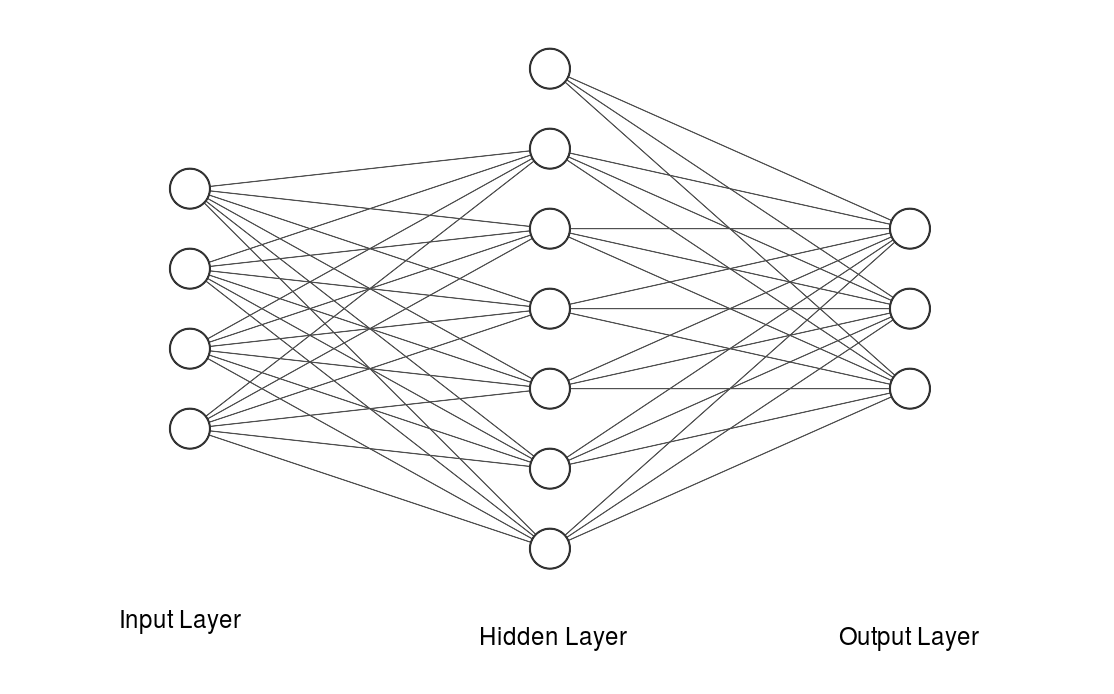
\includegraphics[width=1\textwidth]{FC.png}
%\end{figure}

\noindent\textcolor{red}{\textbf{变量说明:}}
\begin{itemize}
  \item 以零为下角标的变量为 偏置(bias)。
  \item $x$ 表示输入数据(一个训练样本为一个行向量),$y$ 表示标签(one-hot 编码,为一个行向量),$s$~为求和值,$a$~为激活值。
  \item $x^i_j$ 的上标表示第 i 行数据样本,下标表示该行数据样本的第 j 个值。
  \item $x,s,a$~若无下角标,则表示向量化。
  \item 多分类标签 $y$ 采用 one-hot 编码。
\end{itemize}

\begin{definition}
\textcolor{red}{向量上标+ 运算符}:为该向量添加Bias列,具体在第0列添加全1。\\
\textcolor{red}{~~~~~~~~~~~~~~~~向量上标- 运算符}:为该向量删去Bias列,具体删除第0列。
\end{definition}
\begin{example}
~~~~~~~$a = \left(
 \begin{matrix}
   a & b & c \\
   d & e & f \\
   g & h & i
  \end{matrix}
  \right) $~~~~~~
  $a^+ = \left(
\begin{matrix}
   1 & a & b & c \\
   1 & d & e & f \\
   1 & g & h & i
  \end{matrix}
  \right) $~~~~~~
  $a^- = \left(
\begin{matrix}
    b & c \\
    e & f \\
    h & i
  \end{matrix}
  \right) $
\end{example}
\begin{definition}
\textcolor{red}{同维矩阵对应位置相乘运算}:$A\circ B$ .
\end{definition}
\textbf{输入层三个神经元,一个隐藏层六个神经元,输出层三个神经元(三分类)为例。激活函数以逻辑函数,损失函数以均方差损失为例。}

\begin{overpic}[width=0.82\textwidth]{FC.png}

    \put(12,45){\small\bfseries\color{blue}{$x_0^0$}}

    \put(15.3,44.8){\footnotesize\bfseries$+1$}

    \put(12,38){\small\bfseries \color{blue}{$x_1^0$}}

    \put(12,31){\small\bfseries \color{blue}{$x_2^0$}}

    \put(12,24){\small\bfseries \color{blue}{$x_3^0$}}

    \put(50,58){\small\bfseries \color{red}{$a_0^1$}}

    \put(47.8,55.5){\footnotesize\bfseries $+1$}

    \put(47,51){\small\bfseries \color{red}{$s_1^1|a_1^1$}}

    \put(47,44){\small\bfseries \color{red}{$s_2^1|a_2^1$}}

    \put(47,37){\small\bfseries \color{red}{$s_3^1|a_3^1$}}

    \put(47,30){\small\bfseries \color{red}{$s_4^1|a_4^1$}}

    \put(47,23){\small\bfseries \color{red}{$s_5^1|a_2^1$}}

    \put(47,16){\small\bfseries \color{red}{$s_6^1|a_2^1$}}

    \put(84,41){\small\bfseries $s_1^2|a_1^2$}

    \put(84,34){\small\bfseries $s_2^2|a_2^2$}

    \put(84,27){\small\bfseries $s_3^2|a_3^2$}

    \put(30, 47){\small\bfseries \color{green}{$w_{01}^1$}}

    \put(33, 44){\small\bfseries \color{green}{$w_{11}^1$}}

    \put(37, 43){\small\bfseries \color{green}{$w_{21}^1$}}

    \put(41, 43){\small\bfseries \color{green}{$w_{31}^1$}}

    \put(64, 49){\small\bfseries \color{green}{$w_{01}^2$}}

    \put(64, 45){\small\bfseries \color{green}{$w_{11}^2$}}

    \put(64, 41.2){\small\bfseries \color{green}{$w_{21}^2$}}

    \put(64, 37.4){\small\bfseries \color{green}{$w_{31}^2$}}

    \put(64, 33.6){\small\bfseries \color{green}{$w_{41}^2$}}

    \put(64, 29.8){\small\bfseries \color{green}{$w_{51}^2$}}

    \put(64, 26){\small\bfseries \color{green}{$w_{61}^2$}}

    \put(12, 18){\normalsize\bfseries $\big(x^{(0)}\big)^+$}

    \put(30, 12){\normalsize\bfseries {$w^{(1)}$}}

    \put(42, 7){\normalsize\bfseries {$s^{(1)}|\big(a^{(1)}\big)^+$}}

    \put(64, 13){\normalsize\bfseries {$w^{(2)}$}}

    \put(80, 18){\normalsize\bfseries $s^{(2)}|a^{(2)}$}
\end{overpic}

\noindent\textbf{作用过程:}
\begin{enumerate}
  \item 向前传播计算误差:
  \begin{align*}
    & \big(x^{(0)}\big)^+w^{(1)}=s^{(1)},~~~\sigma(s^{(1)})=a^{(1)}\\
    & \big(a^{(1)}\big)^+w^{(2)}=s^{(2)},~~~\sigma(s^{(2)})=a^{(2)} \\
    & Loss~~~L=\frac{1}{2}\sum_{k=1}^{3}(a^{(2)}_k-y_k)^2
  \end{align*}

    \noindent假设有 1 个训练样本:
  \begin{enumerate}[(1)]
    \item $x$  的维度就是 $1\times 3$。
    \item $x^+$  的维度就是 $1\times 4$。
    \item $w^{(1)}$ 的维度就是 $4 \times 6$。
    \item $s^{(1)}$ 的维度就是 $1\times 6$。
    \item $a^{(1)}$ 的维度就是 $1 \times 6$。
    \item $\big(a^{(1)}\big)^+$ 的维度就是 $1 \times 7$。
    \item $w^{(2)}$ 的维度就是 $7 \times 3$。
    \item $s^{(2)}$ 的维度就是 $1\times 3$。
    \item $a^{(2)}$ 的维度就是 $1 \times 3$。 (输出层)
  \end{enumerate}
  \item 误差反向传播计算权值梯度:
  \begin{enumerate}[(1)]
    \item 输出层权值梯度:
      \begin{align*}
    Loss,~~~L&=\frac{1}{2}\sum_{i=1}^{K}(a^{(2)}_i-y_i)^2\\
    \frac{\partial L}{w^{(2)}_{ik}}&=\frac{\partial}{\partial w^{(2)}_{ik}}\frac{1}{2}\sum_{i=1}^{K}(a^{(2)}_i-y_i)^2\\
    &=\big(\sigma(s^{(2)}_k)-y_k\big)\sigma(s^{(2)}_k)\big(1-\sigma(s^{(2)}_k)\big)\frac{\partial s^{(2)}_k}{\partial w^{(2)}_{ik}}\\
    &=\big(\sigma(s^{(2)}_k)-y_k\big)\sigma(s^{(2)}_k)\big(1-\sigma(s^{(2)}_k)\big)\big(a^{(1)}_i\big)^+\\
    \text{令,}~~\delta^{(2)}_k&=\big(\sigma(s^{(2)}_k)-y_k\big)\sigma(s^{(2)}_k)\big(1-\sigma(s^{(2)}_k)\big)\\
    &=\big(a^{(2)}_k-y_k\big)a^{(2)}_k\big(1-a^{(2)}_k\big)\\
    \text{则,}\frac{\partial L}{w^{(2)}_{ik}}&=\delta^{(2)}_k\big(a^{(1)}_i\big)^+
  \end{align*}
    \item 隐藏层权值梯度:
    \begin{align*}
       \frac{\partial L}{\partial w^{(1)}_{ij}}&=\frac{\partial}{\partial w^{(1)}_{ij}}\frac{1}{2}\sum_{k\in K}(a^{(2)}_k-y_k)^2\\
       &=\sum_{k\in K}(a^{(2)}_k-y_k)\frac{\partial \sigma(s^{(2)}_k)}{\partial  w^{(1)}_{ij}}\\
       &=\sum_{k\in K}(a^{(2)}_k-y_k)\sigma(s^{(2)}_k)\big(1-\sigma(s^{(2)}_k)\frac{\partial s^{(2)}_k}{\partial  w^{(1)}_{ij}}\\
       &=\sum_{k\in K}(a^{(2)}_k-y_k)\sigma(s^{(2)}_k)\big(1-\sigma(s^{(2)}_k)\frac{\partial s^{(2)}_k}{\partial  a^{(1)}_{j}}\frac{\partial a^{(1)}_{j}}{\partial  w^{(1)}_{ij}}\\
       &=\sum_{k\in K}(a^{(2)}_k-y_k)\sigma(s^{(2)}_k)\big(1-\sigma(s^{(2)}_k)w^{(2)}_{jk}\frac{\partial a^{(1)}_{j}}{\partial  w^{(1)}_{ij}}\\
       &=\frac{\partial a^{(1)}_{j}}{\partial  w^{(1)}_{ij}}\sum_{k\in K}(a^{(2)}_k-y_k)\sigma(s^{(2)}_k)\big(1-\sigma(s^{(2)}_k)w^{(2)}_{jk}\\
       &=a^{(1)}_j\big(1-a^{(1)}_j\big)\frac{\partial s^{(1)}_j}{w^{(1)}_{ij}}\sum_{k\in K}\delta^{(2)}_kw^{(2)}_{jk}\\
       &=a^{(1)}_j\big(1-a^{(1)}_j\big)\big(x^{(0)}_i\big)^+\sum_{k\in K}\delta^{(2)}_kw^{(2)}_{jk}\\
       \text{令, }~~~ \delta^{(1)}_j &= a^{(1)}_j(1-a^{(1)}_j)\sum_{k \in K} \delta^{(2)}_kw^{(2)}_{jk}\\
       \text{则,} \frac{\partial L}{\partial w^{(1)}_{ij}}&= \delta^{(1)}_j \big(x_i^{(0)}\big)^+
    \end{align*}
  \end{enumerate}


  \item 更新权值:
  \begin{align*}
    W = W -\eta \frac{\partial Loss}{\partial W}
  \end{align*}
\end{enumerate}



\subsubsection{作用过程推广}

\noindent\textbf{用户指定神经网络相关参数:}
\begin{table}[!h]
\resizebox{\textwidth}{!}{
\begin{tabular}{|l|l|l|}
\hline
变量名称        & 符号    & 备注                                                                                                       \\ \hline\hline
训练样本维度      & $N_t$ &                                                                                                          \\ \hline
训练样本数量      & $N_T$ &                                                                                                          \\ \hline
隐藏层数       & $N$ & 包含N个隐藏层                                                                                                       \\ \hline
第i层神经元个数 & $N^{(i)}$ & \begin{tabular}[c]{@{}l@{}}$i=0,1,\cdots,N,N+1$\\$i=N+1$, 输出层,$N^i=K$\\ \textcolor{red}{这里定义不带 bias 神经元。}\end{tabular} \\ \hline

第i层的激活函数 & $\sigma^{(i)}$ & 在常用的 sigmoid,tanh,relu,leaky relu 中选择                                                                               \\ \hline
分类类别数       & K     &                                                                                                          \\ \hline
损失函数        & $S_l$ & 在常用的 MeanSquareError,CorssEntropyLoss 中选择                                                                \\ \hline
\end{tabular}}
\end{table}

~\\
\noindent\textbf{常见激活函数:}
\begin{enumerate}
  \item sigmoid
  \begin{align*}
    \sigma(z) &= \frac{1}{1+e^{-z}}\\
    \sigma'(z) &= \sigma(z)(1-\sigma(z))
  \end{align*}

  \item tanh
  \begin{align*}
    \sigma(z) &= \frac{e^z-e^{-z}}{e^z+e^{-z}} = 1- \frac{2e^{-z}}{e^z + e^{-z}}\\
    \sigma'(z) &= 1-\sigma(z)^2
  \end{align*}

  \item relu
  \begin{align*}
    \sigma(z) &= \begin{cases}
                   ~~0, & \mbox{if } z<0 \\
                   ~~z, & \mbox{otherwise}.
                 \end{cases}\\
    \sigma'(z) &= \begin{cases}
                   ~~0, & \mbox{if } z<0 \\
                   ~~1, & \mbox{otherwise}.
                 \end{cases}\\
  \end{align*}

  \item leaky relu
  \begin{align*}
    \sigma(z) &= \begin{cases}
                   ~~z, & \mbox{if } z>0 \\
                   ~~az, & \mbox{otherwise}.
                 \end{cases}\\
    \sigma'(z) &= \begin{cases}
                   ~~1, & \mbox{if } z>0 \\
                   ~~a, & \mbox{otherwise}.
                 \end{cases}\\
  \end{align*}

  \item softmax
  \begin{align*}
    \text{第 i 个类目的概率, }p_i = a^{(N+1)}_i &=\sigma(s^{(N+1)}_i)= \frac{e^{s^{(N+1)}_i}}{\sum_{j=1}^{K} e^{s^{(N+1)}_j}}
  \end{align*}
\begin{align*}
  &\frac{\partial p_i}{\partial s_j}=\frac{\partial\frac{e^{s_i}}{\sum_{k=1}^{N}e^{s_k}}}{\partial s_j}\\
  &f(x) = \frac{g(x)}{h(x)},~~~~~~~~~f'(x)=\frac{g'(x)h(x)-h'(x)g(x)}{h^2(x)}\\
  &g(x)=e^{s_i},~~~~~~~~~h(x)=\sum_{k=1}^{N}e^{s_k}
\end{align*}
\begin{align*}
  &i==j&&i\neq j\\
  \frac{\partial\frac{e^{s_i}}{\sum_{k=1}^{N}e^{s_k}}}{\partial s_j}&=\frac{e^{s_i} \sum_{k=1}^{N} e^{s_k}-e^{s_j}e^{s_i}}{\big(\sum_{k=1}^{N}e^{s_k}\big)^2}&\frac{\partial\frac{e^{s_i}}{\sum_{k=1}^{N}}}{\partial s_j}&=\frac{0-e^{s_j}e^{s_i}}{\big(\sum_{k=1}^{N}e^{s_k}\big)^2}\\
  &=\frac{e^{s_i}\big(\sum_{k=1}^{N}e^{s_k}-e^{s_j}\big)}{\big(\sum_{k=1}^{N}e^{s_k}\big)^2}&&=-\frac{e^{s_i}}{\sum_{k=1}^{N}e^{s_k}}\frac{e^{s^j}}{\sum_{k=1}^{N}e^{s_k}}\\
  &=p_i(1-p_j)&&=-p_ip_j
\end{align*}
\noindent\textbf{总结:}\\
$$
\delta_{ij}=
\begin{cases}
1& i==j\\
0& i\neq j
\end{cases}
$$
$~~~~~~~~~~~~~~~~~~~~~~~~~~~~~~\Rightarrow$
$$\frac{\partial p_i}{\partial s_j}=p_i(\delta_{ij}-p_j)$$
\end{enumerate}

~\\
\noindent\textbf{常见损失函数:}
\begin{enumerate}
  \item Mean Square Error
  \begin{align*}
    Loss(z,y) &=\frac{1}{2} \sum_{i=1}^{K}(z_i-y_i)^2\\
    \frac{\partial Loss}{\partial z} & = (z-y)  ~~~~~~\text{向量相减}
  \end{align*}
  \item Cross Entropy Loss
  \begin{align*}
    Loss(z,y) &= -\sum_{i=1}^{K}y_i\log z_i=-y_k\log z_k (\text{one-hot 只有第k个分量为 1})\\
    \frac{\partial Loss}{\partial z} &=-\frac{y}{z}  ~~~~~~\text{向量相除}
  \end{align*}
\end{enumerate}
~\\

\noindent \textcolor{red}{一般如果多分类问题输出层使用 CrossEntropy 损失,并用 Softmax 激活。\\因为有:\\$$\frac{\partial Loss(a^{(N+1)}, y)}{\partial s^{(N+1)}_j} = a^{(N+1)}_j -y_j$$
}

~\\
\noindent\textbf{推导:}
\begin{align*}
  \frac{\partial Loss(a^{(N+1)}, y)}{\partial s^{(N+1)}_j} & = \sum_{i=1}^{K} \frac{\partial Loss(a^{(N+1)}, y)}{\partial a_i}\frac{\partial a_i}{\partial s_j}\\
  & = -\sum_{i=1}^{K}\frac{y_i}{a_i}\frac{\partial a_i}{\partial s_j}\\
  &= \big(-\frac{y_i}{a_i}\frac{\partial a_i}{\partial s_j}\big)_{i=j}-\sum_{i=1,i\neq j}^{K}\frac{y_i}{a_i}\frac{\partial a_i}{\partial s_j}\\
  &= -\frac{y_j}{a_j}a_j(1-a_j)-\sum_{i=1,i\neq j}^{K}\frac{y_i}{a_i}\cdot -a_ia_j\\
  &=-y_j+y_ja_j+\sum_{i=1,i\neq j}^{K}y_ia_j\\
  & = -y_j+a_j\sum_{i=1}^{K}y_i\\
  & = a^{(N+1)}_j-y_j
\end{align*}

~\\
\noindent \textbf{变量说明:}

\begin{table}[!h]
\resizebox{\textwidth}{!}{
\begin{tabular}{|l|l|l|}
\hline
变量          & 含义           & 备注                                                                                                                           \\ \hline
$X$           & 输入训练样本       & 维度 $N_T\times N_t$,相当于激活值矩阵$A^{(0)}$.                                                                        \\ \hline
$X^+$           & 输入训练样本加偏置列       & 维度 $N_T\times (N_t+1)$,相当于激活值矩阵$\big(A^{(0)}\big)^+$.                                                                        \\ \hline
$S^{(i)}$   & 第 i 层求和值矩阵 & 维度 $N_T\times N^{(i)}$, $i=1,\cdots,N,N+1$.                                                                                \\ \hline
$A^{(i)}$   & 第 i 层激活值矩阵 & 维度 $N_T\times N^{(i)}$, $i=0,1,\cdots,N,N+1$.                                                                              \\ \hline
$\big(A^{(i)}\big)^+$   & 第 i 层激活值矩阵加偏置列 & 维度 $N_T\times (N^{(i)}+1)$, $i=0,1,\cdots,N$.                                                                              \\ \hline
$W^{(i)}$   & 第 i 层权值矩阵  & 维度 $N^{(i-1)}\times N^{(i)}$, $i=1,\cdots,N,N+1$.                                                                                                  \\ \hline
$W^{(N+1)}$ & 输出层权值矩阵      & 维度 $N^{(N)}\times K$, 标签有 K 个类目。                                                                                     \\ \hline
$W_b^{(i)}$   & 第 i 层权值偏置矩阵  & 维度 $(N^{(i-1)}+1)\times N^{(i)}$, $i=1,\cdots,N,N+1$.                                                                                                  \\ \hline
$W_b^{(N+1)}$   &输出层权值偏置矩阵  & 维度 $(N^{(N)}+1)\times K$, 标签有 K 个类目。                                                                                                 \\ \hline
$S^{(N+1)}$ & 输出层求和值矩阵     & 维度 $N_T\times K $.                                                                                                           \\ \hline
$A^{(N+1)}$ & 输出层激活值矩阵     & 维度 $N_T\times K $.                                                                                                           \\ \hline
$Y$ & 训练数据标签 & 维度 $N_T \times K$ (ONE-HOT).\\ \hline
$\Delta^{(i)}$ & 第 i 层的反向传播中间变量矩阵 & 维度 $N_T \times N^{(i)}$, $i=1,\cdots,N,N+1$.\\ \hline
$\Delta^{(N+1)}$ & 输出层反向传播中间变量矩阵 & 维度 $N_T \times K$.\\ \hline
\end{tabular}}
\end{table}

\paragraph{神经网络向前传播}
\begin{align*}
   \big(A^{(0)}\big)^+W_b^{(1)}=S^{(1)}\stackrel{\sigma+b}{\longrightarrow} \big(A^{(1)}\big)^+&\Rightarrow \cdots \Rightarrow \cdots \\
  & \Rightarrow \big(A^{(N-1)}\big)^+W_b^{(N)}=S^{(N)} \stackrel{\sigma+b}{\longrightarrow}\big(A^{(N)}\big)^+  \\
  & \Rightarrow \big(A^{(N)}\big)^+W_b^{(N+1)}=S^{(N+1)}\stackrel{\sigma}{\longrightarrow} A^{(N+1)} \\
  & \Rightarrow ~\mathcal{L}(A^{(N+1)},Y)
\end{align*}
\paragraph{神经网络反向传播}
\begin{enumerate}
  \item 输出层权值求导:
  \begin{align*}
  \nabla_{W_b^{(N+1)}}\mathcal{L}(A^{(N+1)},Y) &= \frac{1}{N_T}(A^{(N)^+})^T\Delta^{(N+1)}~~~~~~\text{(矩阵化)}\\
  \Delta^{(N+1)}& = \frac{\partial \mathcal{L}(A^{(N+1)}, Y)}{\partial A^{(N+1)}}\circ\sigma'(S^{(N+1)})\\
  \text{当输出层使用 Soft}&\text{max+CrossEntropy 时:}\\
  \Delta^{(N+1)} &= A^{(N+1)} - Y
\end{align*}
  \item 隐藏层权值求导:
\begin{align*}
  \nabla_{W_b^{(N)}}\mathcal{L}(A^{(N+1)},Y)&= \frac{1}{N_T}\big(A^{(N-1)^+}\big)^T\Delta^{(N)}\\
                                \text{令:}       \Delta^{(N)} &=  \big(\Delta^{(N+1)}(W^{(N+1)})^T\big)\circ \sigma'^{(N)}(S^{(N)})\\
    \text{\textcolor{red}{\sffamily扩展:~对于第 i 个隐藏层}}&\text{\textcolor{red}{\sffamily的权值矩阵的梯度为($i=1,2,\cdots,N.$):}}\\
    \nabla_{W_b^{(i)}}\mathcal{L}(A^{(N+1)},Y)&= \frac{1}{N_T}\big(A^{(i-1)^+}\big)^T\Delta^{(i)}\\
                                \text{令:}       \Delta^{(i)} &=  \Delta^{(i+1)}(W^{(i+1)})^T\circ\sigma'^{(i)}(S^{(i)})
\end{align*}
\end{enumerate}

\paragraph{全连接神经网络结构图}

~\\
\\
\begin{overpic}[width=1\textwidth]{FCNN2.png}
\put(1,37.55){\colorbox{yellow}{\tiny \sffamily +1}}
\put(19.9,46){\colorbox{yellow}{\tiny \sffamily +1}}
\put(38.78,54.45){\colorbox{yellow}{\tiny \sffamily +1}}
\put(57.6,54.45){\colorbox{yellow}{\tiny \sffamily +1}}
\put(76.5,46){\colorbox{yellow}{\tiny \sffamily +1}}

%\put(76.5,51){$\stackrel{forward}{\longrightarrow}$}
%\put(19.9,51){\colorbox{green}{\tiny \sffamily +1}}
%\put(76.5,8){\colorbox{yellow}{\tiny \sffamily +1}}
%\put(19.9,8){\colorbox{yellow}{\tiny \sffamily +1}}


\put(0,0){\tiny \sffamily Input Layer 0}
\put(17,0){\tiny \sffamily Hidden Layer 1}
\put(30,0){\tiny \sffamily $\cdots$}
\put(36,0){\tiny \sffamily Hidden Layer $l$}
\put(54,0){\tiny \sffamily Hidden Layer $l$+1}
\put(67.8,0){\tiny \sffamily $\cdots$}
\put(72,0){\tiny \sffamily Hidden Layer $N$-1}
\put(93,0){\tiny \sffamily Output Layer N}

\put(30,38.1){\tiny \sffamily $\cdots$}
\put(30,33.1){\tiny \sffamily $\cdots$}
\put(30,29.1){\tiny \sffamily $\cdots$}
\put(30,24.1){\tiny \sffamily $\cdots$}
\put(30,19.1){\tiny \sffamily $\cdots$}

\put(67.8,38.1){\tiny \sffamily $\cdots$}
\put(67.8,33.1){\tiny \sffamily $\cdots$}
\put(67.8,29.1){\tiny \sffamily $\cdots$}
\put(67.8,24.1){\tiny \sffamily $\cdots$}
\put(67.8,19.1){\tiny \sffamily $\cdots$}

%\put(44.7,30){\tiny \sffamily $\cdots$}
%\put(44.7,35){\tiny \sffamily $\cdots$}
%\put(44.7,40){\tiny \sffamily $\cdots$}
%\put(44.7,45){\tiny \sffamily $\cdots$}
%\put(44.7,50){\tiny \sffamily $\cdots$}
%
%\put(0,55){\small\bfseries\color{blue}{$X_{N_T\times (N_t+1)}$}}
%\put(10,65){\tiny\bfseries\color{red}{$\big(s^{(0)}\big)_{N^0\times z}|\big(a^{(0)}\big)_{(N^0+1)\times 1}$}}
%\put(8,15){\tiny\bfseries\color{red}{$w^{(0)}\big)_{(N_t+1)\times N_0}$}}
\end{overpic}



~\\
\newpage
\noindent\textbf{神经网络张量流:}
\begin{table}[!h]
\resizebox{\textwidth}{!}{
\begin{tabular}{|c|c|c|c|}
\hline
前向传播          & 维度                        & 反向传播                                                 & 维度                                  \\ \hline \hline
X             & $N_T\times (N_t+1)$       & LOSS                                               & Scalar                           \\ \hline
$S^{(1)}$     & $N_T\times N^{(1)}$       & $\Delta^{(N+1)}$                                     & $N_T\times K$                       \\ \hline
$(A^{(1)})^+$     & $N_T\times (N^{(1)}+1)$     & $\nabla_{W^{(N+1)}}\mathcal{L}$   & $(N^{(N)}+1)\times K$           \\ \hline
$S^{(2)}$     & $N_T\times N^{(2)}$       & $\Delta^{(N)}$                                   & $N_T\times (N^{(N)}+1)$         \\ \hline
$(A^{(2)})^+$     & $N_T\times (N^{(2)}+1)$     & $\nabla_{W^{(N)}}\mathcal{L}$ & $(N^{(N-1)}+1)\times N^{(N)}$ \\ \hline
$\vdots$       & $\vdots$                   & $\vdots$                                              & $\vdots$                             \\ \hline
$S^{(N)}$ & $N_T\times N^{(N)}$   & $\Delta^{(i)}$                                       & $N_T\times (N^{(i)}+1)$             \\ \hline
$(A^{(N)})^+$ & $N_T\times (N^{(N)}+1)$ & $\nabla_{W^{(i)}}\mathcal{L}$     & $(N^{(i-1)}+1)\times N^{(i)}$       \\ \hline
$S^{(N+1)}$   & $N_T\times K$             & $\Delta^{(1)}$                                       & $N_T\times (N^{(1)}+1)$             \\ \hline
$A^{(N+1)}$   & $N_T\times K$             & $\nabla_{W^{(1)}}\mathcal{L}$     & $(N_t+1)\times N^{(1)}$             \\ \hline
\multicolumn{2}{|c|}{comput Loss}              & \multicolumn{2}{c|}{update Weight}                   \\ \hline
\end{tabular}}
\end{table}


\paragraph{优化算法}
\subparagraph{批量梯度下降(Batch Gradient Descent,BGD)}

批量梯度下降法是最原始的形式,它是指在每一次迭代时使用所有样本来进行梯度的更新。
\begin{enumerate}
  \item 对目标函数求导:$$\frac{\Delta J\left(\theta_{0}, \theta_{1}\right)}{\Delta \theta_{j}}=\frac{1}{m} \sum_{i=1}^{m}\left(h_{\theta}\left(x^{(i)}\right)-y^{(i)}\right) x_{j}^{(i)}$$

其中 $i=1,2,\cdots,m$ 表示样本数, $j=0,1$ 表示特征数,这里我们使用了偏置项 $x_0^{(i)}=1$ 。
  \item 每次迭代对参数进行更新: $$\theta_{j}:=\theta_{j}-\alpha \frac{1}{m} \sum_{i=1}^{m}\left(h_{\theta}\left(x^{(i)}\right)-y^{(i)}\right) x_{j}^{(i)}$$
\end{enumerate}

\noindent \textbf{伪码:}\\
$\begin{array}{l}{\text { repeat\{ }} \\ {\qquad \begin{array}{l}{\theta_{j}:=\theta_{j}-\alpha \frac{1}{m} \sum_{i=1}^{m}\left(h_{\theta}\left(x^{(i)}\right)-y^{(i)}\right) x_{j}^{(i)}} \\ { \text { (for }j=0,1)} \\ \} \end{array}}\end{array}$


\begin{enumerate}
  \item 优点:
\begin{itemize}
  \item 一次迭代是对所有样本进行计算,此时利用矩阵进行操作,实现了并行。
  \item 由全数据集确定的方向能够更好地代表样本总体,从而更准确地朝向极值所在的方向。当目标函数为凸函数时,BGD一定能够得到全局最优。
\end{itemize}
  \item 缺点:
\begin{itemize}
  \item 当样本数目 m 很大时,每迭代一步都需要对所有样本计算,训练过程很慢。
\end{itemize}
\end{enumerate}

\subparagraph{随机梯度下降(Stochastic Gradient Descent,SGD)}

随机梯度下降法不同于批量梯度下降,随机梯度下降是每次迭代使用一个样本来对参数进行更新。使得训练速度加快。

\begin{enumerate}
  \item 对一个样本的目标函数求偏导:
        $$\frac{\Delta J^{(i)}\left(\theta_{0}, \theta_{1}\right)}{\theta_{j}}=\left(h_{\theta}\left(x^{(i)}\right)-y^{(i)}\right) x_{j}^{(i)}$$
  \item 参数更新:
$$\theta_{j}:=\theta_{j}-\alpha\left(h_{\theta}\left(x^{(i)}\right)-y^{(i)}\right) x_{j}^{(i)}$$
\end{enumerate}

\noindent \textbf{伪码:}\\
$\begin{array}{l}{\text { repeat\{ }}\\ {\qquad \begin{array}{l}{\text{for}~i=1,\cdots,m\{}\\{~~~~~~~~\theta_{j}:=\theta_{j}-\alpha \left(h_{\theta}\left(x^{(i)}\right)-y^{(i)}\right) x_{j}^{(i)}} \\ { ~~~~~~\text { (for }j=0,1)} \\ ~~~~~~~~\} \\ \} \end{array}}\end{array}$

\begin{enumerate}
  \item 优点:
\begin{itemize}
  \item 由于不是在全部训练数据上的损失函数,而是在每轮迭代中,随机优化某一条训练数据上的损失函数,这样每一轮参数的更新速度大大加快。
\end{itemize}
  \item 缺点:
\begin{itemize}
  \item 准确度下降。由于即使在目标函数为强凸函数的情况下,SGD仍旧无法做到线性收敛。
  \item 可能会收敛到局部最优,由于单个样本并不能代表全体样本的趋势。
  \item 不易于并行实现。
\end{itemize}
\end{enumerate}

\subparagraph{小批量梯度下降(Mini-Batch Gradient Descent, MBGD)}

是对 BGD 以及 SGD 的一个折中办法。其思想是:每次迭代 使用 batch\_size 个样本来对参数进行更新。

这里我们假设 batch\_size=10 ,样本数 m=1000 。

\noindent \textbf{伪码:}\\
$\begin{array}{l}{\text { repeat\{ }}\\ {\qquad \begin{array}{l}{\text { for } \mathrm{i}=1,11,21,31, \ldots, 991 \{}\\{~~~~~~~~\theta_{j}:=\theta_{j}-\alpha \frac{1}{10} \sum_{k=i}^{(i+9)}\left(h_{\theta}\left(x^{(k)}\right)-y^{(k)}\right) x_{j}^{(k)}} \\ { ~~~~~~\text { (for }j=0,1)} \\ ~~~~~~~~\} \\ \} \end{array}}\end{array}$


\begin{enumerate}
  \item 优点:
\begin{itemize}
  \item 通过矩阵运算,每次在一个batch上优化神经网络参数并不会比单个数据慢太多。
  \item 每次使用一个batch可以大大减小收敛所需要的迭代次数,同时可以使收敛到的结果更加接近梯度下降的效果。(比如上例中的30W,设置batch\_size=100时,需要迭代3000次,远小于SGD的30W次)
  \item 可实现并行化。
\end{itemize}
  \item 缺点:
\begin{itemize}
  \item batch\_size的不当选择可能会带来一些问题。

\end{itemize}
\end{enumerate}



\newpage
\subsection{MSVL 语言框架}
\textcolor{red}{数据类型 : 单精度浮点数。}

\subsubsection{辅助函数}
\begin{enumerate}
  \item absolute
  \item min
  \item equal
  \item F2S
  \item sigmoid
  \item tanh
  \item relu
  \item leakyRelu
\end{enumerate}



\subsubsection{矩阵操作函数}
\begin{enumerate}
  \item MatCreate
  \item MatDelete
  \item MatSetVal
  \item MatShape
  \item MatDump
  \item MatAdd
  \item MatSub
  \item MatMul
  \item MatProduct
  \item MatNumMul
  \item MatNumAdd
  \item MatTrans
  \item MatZeros
  \item MatOnes
  \item MatEye
  \item MatRowSum
  \item MatRowMax
  \item MatExp
  \item MatSquare
  \item MatVectorSub
  \item MatVectorDiv
  \item MatCopy
  \item MatPlusRow
  \item MatPlusCol
\end{enumerate}



\subsubsection{矩阵激活函数}

\begin{enumerate}
  \item MatNoneActi
  \item MatSoftmax
  \item MatSigmoid
  \item MatTanh
  \item MatRelu
  \item MatLeakyRelu
\end{enumerate}

\subsubsection{矩阵激活函数导数函数}
\begin{enumerate}
  \item MatDerivationNoneActi   0
  \item MatDerivationSigmoid   1
  \item MatDerivationTanh   2
  \item MatDerivationRelu   3
  \item MatDerivationLeakyRelu   4
  \item MatDerivationSoftmax   5
\end{enumerate}

\subsubsection{损失函数}
\begin{enumerate}
  \item OneHot
  \item MSE
  \item CrossEntropy
\end{enumerate}

\subsubsection{损失函数的导函数}
\begin{enumerate}
  \item MSEDerivative
  \item CrossEntropyDerivative
\end{enumerate}

\subsubsection{神经网络的初始化}
\href{https://blog.csdn.net/z_feng12489/article/details/102856968}{神经网络初始化介绍}
\begin{enumerate}
  \item AllZero initialization
  \item Random initialization
  \item \href{https://blog.csdn.net/z_feng12489/article/details/102913634}{Xavier initialization}
  \item He initialization
\end{enumerate}


相关函数
\begin{enumerate}
  \item gaussrand\_NORMAL  标准高斯随机生成
  \item gaussrand 高斯随机生成
  \item MatInitZero 全零初始化
  \item MatInitRandomNormalization 随机初始化
  \item MatInitXavier Xavier初始化
  \item MatInitHe 凯明初始化
\end{enumerate}


\subsubsection{神经网络用户自定义参数}

\begin{table}[!h]
\resizebox{\textwidth}{!}{
\begin{tabular}{|l|l|l|l|}
\hline
用户自定义参数   & 参数表示               & 数据类型    & 备注                                                                                                                                                                                                                                                                                                 \\ \hline\hline
输入训练样本的数量 & N\_sample          & int     & NULL                                                                                                                                                                                                                                                                                               \\ \hline
单一训练样本的维度 & D\_sample          & int     & NULL                                                                                                                                                                                                                                                                                               \\ \hline
训练样本的真值   & Xval               & float * & 数组长度为 N\_sample * D\_sample                                                                                                                                                                                                                                                                        \\ \hline
训练样本的标签   & Yval               & float * & 数组长度为 N\_sample                                                                                                                                                                                                                                                                                    \\ \hline
权值初始化方式   & Style\_initWeight  & int     & \begin{tabular}[c]{@{}l@{}}0  -\textgreater 全0初始化					\\ 1  -\textgreater 随机初始化\\ 2  -\textgreater Xavier初始化\\ 3  -\textgreater 何凯明初始化\end{tabular}                                                                                                                                                \\ \hline
神经网络隐藏层层数 & N\_hidden          & int     & 注意:这里是隐藏层层数。                                                                                                                                                                                                                                                                                       \\ \hline
各层神经元个数   & N\_layerNeuron     & int *   & 数组长度为 0(输入层),1,...,N\_hidden,N\_hidden+1(输出层).                                                                                                                                                                                                                                                     \\ \hline
各层激活函数    & Nstr\_ActiFsHidden & int *   & \begin{tabular}[c]{@{}l@{}}数组长度为 0(输入层),1,...,N\_hidden,N\_hidden+1(输出层).\\ 取值的映射关系:\\ 0  -\textgreater no activation(input layer)\\ 1  -\textgreater sigmoid\\ 2  -\textgreater tanh\\ 3  -\textgreater relu\\ 4  -\textgreater leaky relu\\ 5  -\textgreater softmax (output layer)\end{tabular} \\ \hline
分类类别数     & N\_out             & int     & NULL                                                                                                                                                                                                                                                                                               \\ \hline
输出层损失函数   & Nstr\_LossF        & int     & \begin{tabular}[c]{@{}l@{}}取值映射关系:\\ 0  -\textgreater MSE\\ 1  -\textgreater CE\end{tabular}                                                                                                                                                                                                       \\ \hline
\end{tabular}}
\end{table}


\subsubsection{神经网络的运算所需空间变量及创建所需空间函数}
\begin{table}[!h]
\resizebox{\textwidth}{!}{
\begin{tabular}{|l|l|l|l|}
\hline
神经网络的运算所需空间变量 & 参数表示                 & 数据类型  & 备注                                                                                                                   \\ \hline
神经网络激活值矩阵     & P\_ActiMat           & Mat * & 列表索引i=0(输入层),1,...,N\_hidden,N\_hidden+1(输出层)                                                                        \\ \hline
神经网络激活值矩阵加偏置列 & P\_ActiMatPlus       & Mat * & \begin{tabular}[c]{@{}l@{}}列表索引i=0(输入层),1,...,N\_hidden\\ 加偏置列 偏置列全部置1.输出层不需要Plus\end{tabular}                       \\ \hline
神经网络求和矩阵      & P\_SumMat            & Mat * & \begin{tabular}[c]{@{}l@{}}列表索引i=0(输入层),1,...,N\_hidden,N\_hidden+1(输出层)\\ i=0 时输入层求和矩阵行列置零 无实际含义\end{tabular}       \\ \hline
神经网络权值矩阵      & P\_WeightMat         & Mat * & \begin{tabular}[c]{@{}l@{}}列表索引i=0(输入层),1,...,N\_hidden,N\_hidden+1(输出层)\\ i=0 时输入层求和矩阵行列置零 无实际含义\end{tabular}       \\ \hline
\rowcolor{yellow}神经网络权值偏置矩阵    & P\_WeightBiasMat     & Mat*  & \begin{tabular}[c]{@{}l@{}}列表索引i = 0(输入层), 1, ..., N hidden,N hidden + 1(输出层)\\ i = 0 时输入层求和矩阵行列置零无实际含义\end{tabular} \\ \hline
训练数据标签        & Mat\_oneHot          & Mat   & row=N\_sample col=N\_out                                                                                             \\ \hline
反向传播中间变量矩阵    & P\_DeltaMat          & Mat * & \begin{tabular}[c]{@{}l@{}}列表索引i=0(输入层),1,...,N\_hidden,N\_hidden+1(输出层)\\ i=0 时输入层求和矩阵行列置零 无实际含义\end{tabular}       \\ \hline
权值偏置矩阵导数变量矩阵  & P\_NablaWbMat        & Mat*  & \begin{tabular}[c]{@{}l@{}}列表索引i = 0(输入层), 1, ..., N hidden,N hidden + 1(输出层)\\ i = 0 时输入层求和矩阵行列置零无实际含义\end{tabular} \\ \hline
激活函数对求和值导数矩阵  & P\_ActiFunDerivation & Mat*  & \begin{tabular}[c]{@{}l@{}}列表索引i = 0(输入层), 1, ..., N hidden,N hidden + 1(输出层)\\ i = 0 时输入层求和矩阵行列置零无实际含义\end{tabular} \\ \hline
\end{tabular}}
\end{table}
\newpage
\noindent \textbf{创建所需空间函数:}
\begin{enumerate}
  \item SpaceCreateActi  创建激活值矩阵所需空间
  \item SpaceCreateActiPlus  创建激活值Plus矩阵所需空间
  \item SpaceCreateSum   创建求和值矩阵所需空间
  \item SpaceCreateWeight   创建权值矩阵所需空间
  \item SpaceCreateWeightBias  创建权值偏置矩阵所需空间
  \item SpaceCreateDelta   创建反向传播中间变量矩阵所需空间
\end{enumerate}


\subsubsection{初始化神经网络}
\noindent\textbf{函数:}
\begin{enumerate}
  \item NNinit
\end{enumerate}

\noindent\textbf{说明:}
\begin{enumerate}
  \item 输入数据喂入激活值(plus)矩阵
  \item 标签数据喂入矩阵并且进行独热编码
  \item 选择常用的初始化方式进行权值初始化
\end{enumerate}


\newpage
\subsubsection{神经网络前向传播}
\begin{table}[!h]
\resizebox{\textwidth}{!}{
\begin{tabular}{|l|l|l|l|}
\hline
神经网络向前传播所需参数变量 & 参数表示               & 数据类型  & 备注                                                                                                                                                                                                                                                                                               \\ \hline\hline
神经网络激活值矩阵      & P\_ActiMat         & Mat * & 列表索引i=0(输入层),1,...,N\_hidden,N\_hidden+1(输出层)                                                                                                                                                                                                                                                    \\ \hline
神经网络激活值矩阵加偏置列  & P\_ActiMatPlus     & Mat * & \begin{tabular}[c]{@{}l@{}}列表索引i=0(输入层),1,...,N\_hidden\\ 加偏置列 偏置列全部置1.输出层不需要Plus\end{tabular}                                                                                                                                                                                                   \\ \hline
神经网络求和矩阵       & P\_SumMat          & Mat * & \begin{tabular}[c]{@{}l@{}}列表索引i=0(输入层),1,...,N\_hidden,N\_hidden+1(输出层)\\ i=0 时输入层求和矩阵行列置零 无实际含义\end{tabular}                                                                                                                                                                                   \\ \hline
神经网络权值偏置矩阵     & P\_WeightBiasMat   & Mat * & \begin{tabular}[c]{@{}l@{}}列表索引i = 0(输入层), 1, ..., N hidden,N hidden + 1(输出层)\\ i = 0 时输入层求和矩阵行列置零无实际含义\end{tabular}                                                                                                                                                                             \\ \hline
训练数据标签         & Mat\_oneHot        & Mat   & row=N\_sample col=N\_out                                                                                                                                                                                                                                                                         \\ \hline
神经网络隐藏层层数      & N\_hidden          & int   & 注意:这里是隐藏层层数。                                                                                                                                                                                                                                                                                     \\ \hline
各层激活函数         & NStr\_ActiFsHidden & int * & \begin{tabular}[c]{@{}l@{}}数组长度为 0(输入层),1,...,N hidden,N hidden+1(输出层).\\ 取值的映射关系:\\ 0 -\textgreater{}no activation(input layer)\\ 1 -\textgreater{}sigmoid\\ 2 -\textgreater{}tanh\\ 3 -\textgreater{}relu\\ 4 -\textgreater{}leaky relu\\ 5 -\textgreater{}softmax (output layer)\end{tabular} \\ \hline
输出层损失函数        & Nstr\_LossF        & int   & \begin{tabular}[c]{@{}l@{}}取值映射关系:\\ 0 -\textgreater{}MSE\\ 1 -\textgreater{}CE\end{tabular}                                                                                                                                                                                                     \\ \hline
\end{tabular}}
\end{table}
\begin{enumerate}
  \item MatActivate 激活函数选择函数
  \item LossFunction 损失函数选择函数
  \item NNforward 神经网络前向传播函数-返回损失
\end{enumerate}


\subsubsection{神经网络反向传播}
\begin{table}[!h]
\resizebox{\textwidth}{!}{
\begin{tabular}{|l|l|l|l|}
\hline
神经网络反向传播所需参数变量         & 参数表示                 & 数据类型  & 备注                                                                                                                                                                                                                                                                                               \\ \hline\hline
神经网络隐藏层层数              & N\_hidden            & int   & 注意:这里是隐藏层层数                                                                                                                                                                                                                                                                                      \\ \hline
输入样本的数量                & N\_sample            & int   & 样本数量(训练样本)                                                                                                                                                                                                                                                                                       \\ \hline
各层神经元个数                & N\_layerNeuron       & int * & 数组长度为 0(输入层),1,...,N hidden,N hidden+1(输出层)                                                                                                                                                                                                                                                      \\ \hline
神经网络求和矩阵               & P\_SumMat            & Mat * & 列表索引i=0(输入层),1,...,N\_hidden,N\_hidden+1(输出层)                                                                                                                                                                                                                                                    \\ \hline
i=0 时输入层求和矩阵行列置零 无实际含义 & P\_ActiMat           & Mat * & 列表索引i=0(输入层),1,...,N\_hidden,N\_hidden+1(输出层)                                                                                                                                                                                                                                                    \\ \hline
神经网络激活值矩阵加偏置列          & P\_ActiMatPlus       & Mat * & \begin{tabular}[c]{@{}l@{}}列表索引i=0(输入层),1,...,N\_hidden\\ 加偏置列 偏置列全部置1.输出层不需要Plus\end{tabular}                                                                                                                                                                                                   \\ \hline
反向传播中间变量矩阵             & P\_DeltaMat          & Mat * & \begin{tabular}[c]{@{}l@{}}列表索引i = 0(输入层), 1, ..., N hidden,N hidden + 1(输出层)\\ i = 0 时输入层求和矩阵行列置零无实际含义\end{tabular}                                                                                                                                                                             \\ \hline
训练数据标签                 & Mat\_oneHot          & Mat   & row = N\_sample col = N\_out                                                                                                                                                                                                                                                                     \\ \hline
训练数据标签                 & Mat\_oneHot          & Mat   & row=N\_sample col=N\_out                                                                                                                                                                                                                                                                         \\ \hline
各层激活函数                 & NStr\_ActiFsHidden   & int * & \begin{tabular}[c]{@{}l@{}}数组长度为 0(输入层),1,...,N hidden,N hidden+1(输出层).\\ 取值的映射关系:\\ 0 -\textgreater{}no activation(input layer)\\ 1 -\textgreater{}sigmoid\\ 2 -\textgreater{}tanh\\ 3 -\textgreater{}relu\\ 4 -\textgreater{}leaky relu\\ 5 -\textgreater{}softmax (output layer)\end{tabular} \\ \hline
输出层损失函数                & Nstr\_LossF          & int   & \begin{tabular}[c]{@{}l@{}}取值映射关系:\\ 0 -\textgreater{}MSE\\ 1 -\textgreater{}CE\end{tabular}                                                                                                                                                                                                     \\ \hline
激活函数对求和值导数矩阵           & P\_ActiFunDerivation & Mat * & \begin{tabular}[c]{@{}l@{}}列表索引i = 0(输入层), 1, ..., N hidden,N hidden + 1(输出层)\\ i = 0 时输入层求和矩阵行列置零无实际含义\end{tabular}                                                                                                                                                                             \\ \hline
\end{tabular}}
\end{table}

\begin{enumerate}
  \item ActiFunDerivation
  \item LossFunDerivation
  \item NNOuputLayerBackward
  \item NNBackward
\end{enumerate}

\subsubsection{优化算法}

\begin{enumerate}
  \item BGD(批量梯度下降)
  \item SGD(随机梯度下降)
  \item MBGD(小批量梯度下降)
  \item Adam ???
\end{enumerate}

\textcolor{red}{demo 成型,损失减小,可收敛。}


\newpage
\subsection{MSVL 语言框架重构}
\subsubsection{对象结构体}

\begin{enumerate}
  \item 矩阵~结构体
\begin{lstlisting} [language=c]
typedef struct {
	int row, col;      // rowNum and columnNum [int]
	float** element;   // element, two dimensions
}Mat;
\end{lstlisting}
  \item BP单层~结构体
\begin{lstlisting} [language=c]
typedef struct{
	Mat ActiMat;               // active value Matrix without bias column
	Mat ActiMatPlus;           // active value Matrix with bias column
	Mat SumMat;                // sum value Matrix
	Mat WeightMat;             // weight value Matrix without bias row
	Mat WeightBiasMat;         // weight value Matrix with bias row
	Mat DeltaMat;              // backtrack temporary variable Matrix
	Mat NablaWbMat;            // gradient Matrix for weight with bias
	Mat ActiFunDerivationMat;  // active Function Dervation Matrix

	int NeuronNum;             // number of neuron [int]
	int AcitFuncNum;           // active function [int]
}FCLayer;
\end{lstlisting}
  \item BP神经网络~结构体
\begin{lstlisting} [language=c]
typedef struct{
	int CurrentSampleNum;             // number of current samples [int]
	int SampleDimensionNum;    // dimensions(features) of sample [int]
	int HiddenLayerNum;        // number of hidden layer [int]
	int WeightInitWayNum;      // weight initialization mode [int]

	FCLayer *Layer;            // layers of FCNN
	Mat OnehotMat;             // onehot code Matrix

	int ClassificationNum;     // Number of categories classified [int]
	int LossFuncNum;           // loss function [int]
}FCNN;
\end{lstlisting}
  \item 用户自定义参数~结构体
\begin{lstlisting} [language=c]
typedef struct{
    int CompleteSampleNum;		// number of all samples [int]
	int TrainSampleNum;			// number of training samples [int]
	int TestSampleNum;			// number of test samples [int]
	int ValidationNum;			// number of validation samples [int]
	int SampleDimensionNum;    // dimensions(features) of sample [int]
	int HiddenLayerNum;        // number of hidden layer [int]
	int WeightInitWayNum;      // weight initialization mode [int]
	float *XValArray;          // samples features value [float*]
	float *YValArray;          // samples labels value [float*]
	int *NeuronNumArray;       // numbers of every layers Neuron [int*]
	int *ActiFuncNumArray;     // activate functions of every layers [int*]
	int ClassificationNum;     // Number of categories classified [int]
	int LossFuncNum;           // loss function [int]
}Custom;
\end{lstlisting}
%   int OptiAlgNum;            // optimize algorithm [int]
%   float lr;                  // learning rate for optimize algorithm[float]
%   int batch;                 // batch number for optimize algorithm [int]

\item 数据集~结构体
\begin{lstlisting} [language=c]
typedef struct{
	Mat CompleteFeatureDataSet;	// complete featrue Mat for FCNN
	Mat CompleteLabelDataSet;	// complete label Mat without onehot
	Mat CompleteTrainFeature;	// complete featrue Mat for FCNN training
	Mat CompleteTrainLabel;		// complete label Mat without onehot
	Mat *BatchTrainFeature;		// batch featrue Mat for FCNN training [three dimensions]
	Mat *BatchTrainLabel;		// batch label Mat without onehot [three dimensions]
	Mat *BatchTrainLabelOneHot; // batch label Mat with onehot [three dimensions]
	Mat TestFeature;			// featrue Mat for FCNN test
	Mat TestLabel;				// label Mat without onehot
	Mat TestLabelOneHot;        // label Mat with onehot
	//Mat ValidationFeature;	// featrue Mat for FCNN Validation
	//Mat ValidationLabel;		// label Mat withoutone
	

	int CompleteSampleNum;		// number of all samples [int]
	int TrainSampleNum;			// number of training samples [int]
	int TestSampleNum;			// number of test samples [int]
	//int ValidationNum;			// number of validation samples [int]
	int SampleDimensionNum;    // dimensions(features) of sample [int]
	int ClassificationNum;     // Number of categories classified [int]
	int BatchSize;				// batch size for dataset
	int BatchNum;				// number of batch
	int remainder;				// the last batch size
}DataSet;
\end{lstlisting}
\end{enumerate}




\textcolor{red}{\fbox{batch} 机制的实现:建立 \fbox{batch} 结构体,分割数据集,复制到  \fbox{FCNN}  中。}

其中 $\text{TrainSampleNum} = \text{BatchSize}*\text{BatchNum}+\text{remainder}$,当$\text{remainder}=0$时,代表能被整除。

\subsubsection{开发流程}
\begin{enumerate}
  \item 用户自定义参数及总数据录入;
  \item 数据集构建;
  \item 神经网络初始化;
  \item 前向传播构建;
  \item 反向传播构建;
  \item 优化算法构建;
  \item 神经网络训练构建;
  \item 神经网络测试构建。
\end{enumerate}


\paragraph{神经网络用户自定义参数及总数据录入}~目的是将相关参数及总的数据赋值给用户自定义结构体中(其中注意对数组数据的赋值,传引用即可),再将各个参数分发给各个结构体。


\paragraph{数据集构建} ~根据用户输入的数据相关参数将训练测试数据集构建完成。构建路线:
\begin{enumerate}
  \item 根据训练集数据量以及 $\text{Batch\_Size}$ 大小计算并导入相关参数。
  \item 根据整体数据集的各个参数,开辟所需的全部空间。
  \item 将整体数据集数组根据训练测试集数目划分成两个数组,包括训练特征数组和训练标签数组,测试特征数组和测试标签数组。
  \item 再将训练特征数组和训练标签数组划分成若干个块大小的块训练特征数组和块训练标签数组。
  \item 最后将数据喂入到相应的矩阵结构体当中。
\end{enumerate}


\paragraph{神经网络初始化}
\begin{enumerate}
  \item 开辟神经网络所需空间并导入每层相关参数\textcolor{red}{注意创建顺序不可变化。}
  \begin{enumerate}[(1)]
    \item 创建神经网络层空间
    \begin{enumerate}[<1>]
      \item FCLayer
    \end{enumerate}
        \item 导入每层参数
    \begin{enumerate}[<1>]
      \item NeuronNum
      \item AcitFuncNum
    \end{enumerate}
    \item 创建神经网络运算空间
    \begin{enumerate}[<1>]
      \item ActiMat
      \item ActiMatPlus
      \item SumMat
      \item ActiFunDerivationMat
      \item DeltaMat
      \item OnehotMat(FCNN)
    \end{enumerate}
    \item 创建神经网络参数空间\textcolor{red}{(参数空间的大小不随输入神经网络样本大小而改变)}
    \begin{enumerate}[<1>]
      \item WeightMat
      \item WeightBiasMat
      \item NablaWbMat
    \end{enumerate}
  \end{enumerate}
  \item 进行权值初始化
  \begin{enumerate}
    \item WeightMat
    \item WeightBiasMat
  \end{enumerate}
\end{enumerate}



\paragraph{神经网络前向传播求损失} ~神经网络向前传播将小批量输入样本导入神经网络输入层激活值矩阵,并将对应的标签数据进行独热编码,然后进行矩阵运算损失处理得到标量损失值。\textcolor{red}{其中要注意小批量输入样本的数量不一定和已经开辟的神经网络有关矩阵空间的数量相一致,要做检查处理。}

\begin{enumerate}
  \item 小批量余数处理
  \item 输入特征数据拷贝到激活值矩阵
  \item 输入标签独热编码数据拷贝到神经网络独热编码矩阵中
  \item 前向传播矩阵相乘,激活,扩展激活值矩阵
  \item 预测值矩阵与真实值矩阵求损失,返回
\end{enumerate}

\paragraph{神经网络反向传播求梯度} ~神经网络先经过一次正向传播得到损失之后,再求其损失对所有权值偏置的导数得到梯度,用到了\textcolor{red}{反向传播算法}。注意,每一次反向传播是建立在一次正向传播求得损失的基础之上的。

\begin{enumerate}
  \item 输出层反向传播,求得输出层的中间变量矩阵以及权值导数
  \item 隐藏层反向传播,求得各隐藏层的中间变量矩阵以及权值导数
\end{enumerate}